\chapter{Theoretische Grundlagen}

In diesem Kapitel werden die für den Forschungshintergrund und für die Entwicklung des Prototyps wichtigen theoretischen Grundlagen vorgestellt.
Zunächst werden verschiedene Theorien zu Kommunikationsmodellen vorgestellt, auf deren Basis das Modell für diese Anwendung zugrunde liegt.
Im Anschluss daran werden die in der Ludologie beschriebenen Akteure vorgestellt, welche sich in den Probanden dieser Masterarbeitsstudie wiederfinden werden. Allgemein ist bekannt, dass Video- und Computerspiele drei verschiedene Modi haben können: Singleplayer, Multiplayer und Mischformen. Da für den Zweck dieser Studie ein Multiplayer-Spiel konzipiert und umgesetzt wurde, werden im weiteren Verlauf verschiedene Kategorien von Multiplayer-Spielen vorgestellt. Außerdem werden die damit einhergehenden Netzwerkinfrastrukturen vorgestellt, die relevant sind und für die weitere Entwicklung relevant sein könnten.

\section{Kommunikationsmodelle}
[Literatur suchen]
% In der Kommunikationswissenschaft wird die Kommunikation in 2 Arten unterteilt, die Massen- und Individualkommunikation.
[hier spielen dann auch die parameter ne Rolle, die kommunikation anspricht oder enthält]
\subsection{Nach Schulz von Thun}
\subsection{Nach Wazlawik}
\subsection{Nach Rogers}

% [Könnte besser in die Einleitung passen
% \section{Spiele als soziales Medium}
% \cite{depping_trust_2016}
% \cite{gerling_designing_2014}
% \cite{ducheneaut_alone_2006}
% ]

\section{Spielertypen}
Die Kommunikationswissenschaft umfasst zwar den Hauptteil dieser Arbeit, allerdings beinhaltet diese ebenfalls ludologische Aspekte. Dabei geht es um die Lehre über das Spiel (vgl. \cite{ludologie_spielforschung_nodate}). 

Im Hinblick auf die Konzeption und die Entwicklung eines Spiels ist es wichtig, die Eigenschaften des Spielsystems so zu gestalten, dass sich Begeisterung und Engagement bei der gewünschten Zielgruppe hervorrufen. Aus diesem Grund muss zunächst die Zielgruppe in verschiedene Typen eingeteilt werden. In der Ludologie gibt es dafür verschiedene Spielertypen. Zwar ist nicht jeder Mensch ein \say{Spielertyp}, grundsätzlich kann er jedoch über verschiedene Spielelemente angesprochen werden (vgl. \cite{ludologie_spielertypen_nodate}).

\subsection{Nach Bartle}
1996 beschäftigte sich Richard Bartle mit der Frage, welche Spielertypen es in der Ludologie gibt. Dabei ging es zunächst um die Klassifizierungen, welche Ansätze es beim Spielen von sogenannten \ac{MUD}s existieren (vgl. \cite{bartle_hearts_1996}). Diese Klassifizierungen werden noch heute für die Einteilung in Spielertypen genutzt.

Bartle unterscheidet bei der Einteilung der Spielertypen auf zwei unterschiedliche Grundinteressen (vgl. Abbildung \ref{fig:bartle-muds}):

\begin{figure}[ht]
\centering
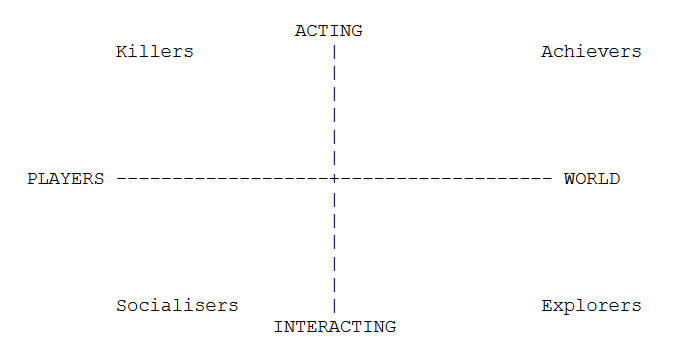
\includegraphics[width=1\linewidth]{content/pictures/basic_interests.PNG}
\caption{Interessen Graph nach Bartle (vgl. \cite{bartle_hearts_1996})}
\label{fig:bartle-muds}
\end{figure}

In X-Achsen-Richtung wird unterschieden, ob der Spieler seine Spielerfahrung über das Verhalten der anderen Mitspieler (Players) oder der Spielwelt (World) bevorzugt. Auf der Y-Achsen-Richtung unterscheidet er, ob der Spieler bevorzugt, selbst einen Einfluss auf die Spielwelt zu geben und diese beeinflusst (Acting) oder ob er in tiefere Interaktion mit der Spielwelt eingehen will (Interacting).

Die daraus resultierenden Typen sind:
\paragraph{Achiever}
Sie sind daran interessiert, auf die Welt einzuwirken, um dadurch in sie eintauchen zu können. Sie wollen das Spiel meistern und dazu bringen, das zu tun, was sie wollen. Ihr Status im Spiel ist ihnen wichtig und die wenige Zeit, die sie dafür benötigt haben.

\paragraph{Explorer}
Sie wollen vom Spiel überrascht werden und mit der Spielwelt interagieren. Die virtuelle Welt löst ein Gefühl des Staunens aus, nach dem sie sich sehnen. Sie sind stolz auf das Wissen über das Spiel, das sie sammeln, und wollen dieses Wissen gerne an neue Spieler weitergeben.

\paragraph{Socialiser}
Sie wollen mit anderen Spielern interagieren. Zumeist erfolgt das über Gespräche, es kann aber auch ungewöhnliche Verhaltensweisen einschließen. Andere Menschen kennenzulernen und mehr über sie zu erfahren, ist für sie wertvoller als für andere. Die Spielwelt ist für sie nur eine Kulisse, für sie sind andere Charaktere fesselnder. Sie sind stolz auf Freundschaften, ihre Kontakte und ihren Einfluss.

\paragraph{Killer}
Sie sind daran interessiert, auf andere Spiele einzuwirken und mit ihnen Dinge zu machen. Im Allgemeinen erfolgt dies ohne das Einverständnis der anderen Spieler. Sie wollen ihre Überlegenheit gegenüber anderen Menschen demonstrieren. Sie sind stolz auf ihren Ruf und oft geübten Kampffähigkeiten.

(vgl. \cite{bartle_hearts_1996}).

\subsection{Erweiterte Einteilungen}
Bartle ist nicht der Einzige, der sich mit Spielertypen auseinandergesetzt hat. Seine Forschung gilt als Fundament, welches in der weiteren Forschung für Diskussionen in der Forschungs- und Game-Design-Community gesorgt hat. 
\begin{quote}
    \textit{
        \enquote{Player types are not a defined concept and any categorization of players or users needs to occur within the context of a particular application or domain. Play-personas are suggested as a useful tool that can be used to put player type research into practice as part of the design process of gamified systems.}
    } 
    (\cite{dixon_player_nodate})
\end{quote}

\paragraph{Dixon} 
stellt Spieler-Personae vor, die wie im \ac{UCD}-Prozess verwendet werden können. Dadurch muss im Designprozess nicht zu sehr zwischen Motivation, Verhalten oder Vorlieben unterschieden werden, da Personae als reichhaltige und erzählerische Darstellung gedacht sind (vgl. \cite{dixon_player_nodate}).

\paragraph{Bateman und Boon}
benutzen in ihrer 2005 erschienen Studie zur Bestimmung des ersten Modells des demografischen Game Designs (DGD1) vier Spielstile, welche sie durch die Hinzunahme der Myers-Briggs Type Indicator (vgl. \cite{noauthor_mbti_nodate}) ableiteten (vgl. \cite{bateman_21st_2005}).
Conquerer (Eroberer), Manager, Wanderer (Wanderer) und Participant (Teilnehmer) waren dabei die vier Spielstile.

In einer zweiten Studie wurden vier hypothetische Spielstile erstellt, welche von einer Studie von Berens 2000 (vgl. \cite{berens_understanding_2000}) abgeleitet wurden (vgl. \cite{bateman_player_2012}). Die resultierenden Stile sind folgende: Logistical, Tactical, Strategic und Diplomatic.

Im Kern sind diese Modelle Ableitungen von Bartles ursprünglicher Metrik (vgl. \cite{ludologie_spielertypen_nodate}).

\paragraph{Yee}
Nick Yee entwickelte empirisch fundiertes Modell zur Beschreibung von Spielmotivationen in Online-Spielen, das bis heute einen großen Einfluss auf die Ludologie hat. Mittels eines faktorenanalytischen Ansatzes untersuchte er eine Vielzahl an Daten aus Online-Umfragen und identifizierte dabei 10 spezifische Motivationsgruppen, die in drei übergeordnete Hauptkategorien gegliedert werden (vgl. Abbildung \ref{fig:nick_yee_motivations}):

\begin{figure}[ht]
\centering
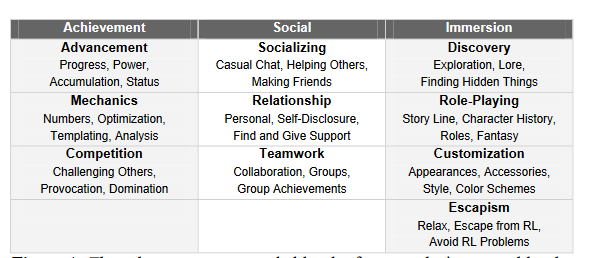
\includegraphics[width=1\linewidth]{content/pictures/nick_yee_categorizations.PNG}
\caption{Motivationsgruppen nach Nick Yee (vgl. \cite{yee_motivations_nodate})}
\label{fig:nick_yee_motivations}
\end{figure}

Die Achievement-Komponente umfasst den Fortschritt im Spiel, sowie das damit einhergehende Verlangen Macht zu erlangen, schnell voranzukommen und Symbole von Reichtum oder Status im Spiel zu erlangen. Außerdem existiert ein Interesse daran, die Mechanik des Spiels zu analysieren, die Regeln und Systeme zu verstehen um die Leistung der Spielfigur zu optimieren. Außerdem ist der Wettbewerb wichtig. Es besteht der Wunsch danach sich mit anderen zu messen und gegen sie anzutreten.

Die soziale Komponente beschreibt dabei die Sozialisierung der Spieler, bei denen sie Interesse daran haben anderen Spielern zu helfen und sich mit ihnen zu Unterhalten. Daraus entstehen Beziehungen, bei denen der Wunsch nahe liegt, dass langfristige und bedeutungsvolle Beziehungen zu anderen aufgebaut werden können. Außerdem ist Teamarbeit gewünscht, um sich gegen andere zu messen und gegen sie anzutreten.

Die Immersions-Komponnete beschreibt das Entdecken in der Spielwelt und dem damit einhergehende finden von Dingen, Wissen zu erlangen, welches den meisten anderen Spielern unbekannt ist. Rollenspiel-Elemente sind dabei besonders wichtig, um den Spielfiguren eine Hintergrundgeschichte zu geben und gemeinsam eine improvisierte Geschichte zu entwickeln. Der Spielavatar sollte auch anpassbar sein, damit der individuelle Geschmack der Spieler in das Spiel einfließen kann. Die Spiel-Welt wird genutzt um von den Problemen der realen-Welt zu entkommen.

\paragraph{weitere Modelle}
Im Zuge der fortschreitenden Forschungen entstanden weitere Modelle wie das Gamer Motivation Model, das auf Basis der Forschung von Nick Yee entwicjelt wurde (vgl. \cite{ludologie_spielertypen_nodate}):

\begin{figure}[ht]
\centering
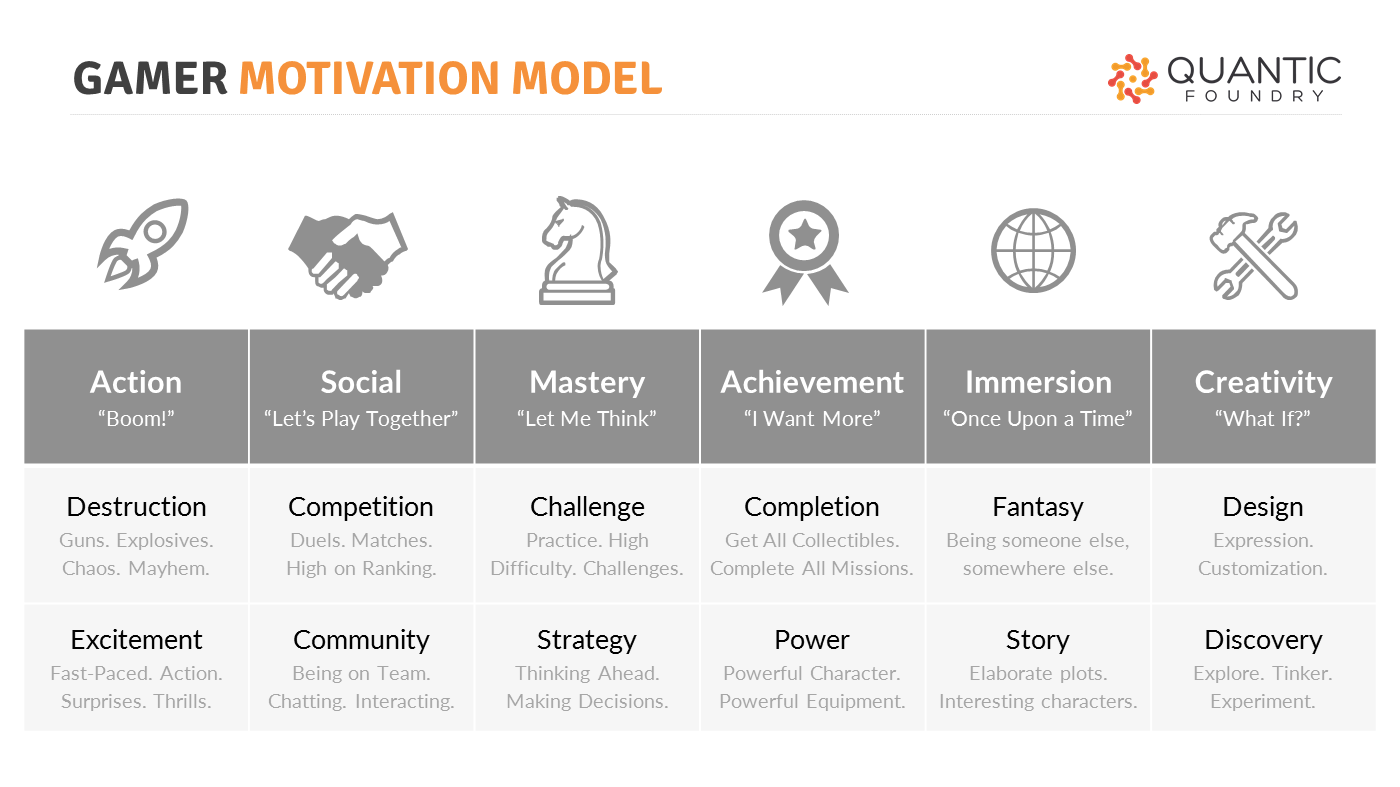
\includegraphics[width=1\linewidth]{content/pictures/gamer_motivations_model.png}
\caption{Gamer Motivation Model der QUANTIC FOUNDRY (vgl. \cite{noauthor_quantic_nodate})}
\label{fig:gamer_motivation_model}
\end{figure}

Ein weiteres Modell, das in der Arbeit von Bateman genannt wird, ist das BRAINHEX-Model, bei dem die verschiedenen Spielertypen in Hexagonaler Anordnung platziert werden (vgl. Abbildung: \ref{fig:brain-hex}):

\begin{figure}[ht]
\centering
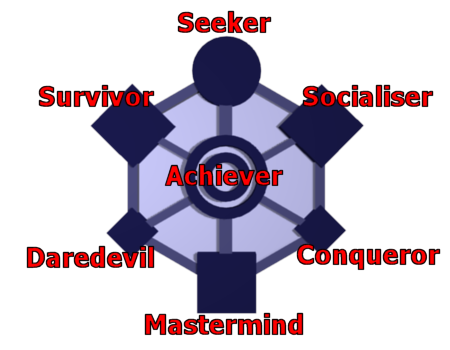
\includegraphics[width=1\linewidth]{content/pictures/brainhex-classes.png}
\caption{Brainhex-Model Darstellung von \cite{noauthor_i_nodate} nach \cite{nacke_brainhex_2013}}
\label{fig:brain-hex}
\end{figure}

% \cite{bartle_hearts_nodate}

% [erwähnen wurde aber rausgelassen, man kann erwähnen, dass es noch weitere klassifizierungen gibt
% \subsection{Das BrainHex-Model}
% \cite{nacke_brainhex_2014}
% ]

% [kommt zu wichtige Begriffe
% \section{Kooperative Gamedesign Pattern}
% \subsection{Was sind Game Pattern}
% \cite{bjork_patterns_2005}

% \subsection{Complementarity}

% \subsection{Synergies}

% \subsection{Abilities}

% \subsection{Shared Goals}

% \subsection{Synergies between goals}

% \subsection{Special Rules for Player of the same Team}

% \subsection{Camera Setting}

% \subsection{Interacting with the same object}

% \subsection{Shared puzzle}

% \subsection{Shared characters}

% \subsection{Special characters targetting lone wolf}

% \subsection{Vocalization}

% \subsection{Limited ressources}

% \subsection{Einflussnahme}
% \cite{emmerich_impact_2017}

% ]
\section{Multiplayer-Spiele}
Im Vergleich zu Einzelspieler-Spielen existieren bei Multiplayer-Spielen nicht nur Unterscheidungen im Genre des Spiels, sondern auch in den Spielrollen (Symmetrie / Asymmetrie) sondern auch in den Spielzeitpunkten (Synchron / Asynchron) wann die Spielteilnehmer an ihrem Sportfortschritt weiter arbeiten. [Hier wäre eine Quelle noch gut]. Auf dem Spielemarkt existieren außerdem Multiplayer-Spiele, die unterschiedliche Medientechniken verwenden. Teilweise werden diese Medientechniken verwendet um eine Cross-Plattform Funktionalität zu gewährleisten (vgl. \cite{noauthor_baldurs_nodate}) oder es ist Teil des Gamedesigns (vgl. \cite{noauthor_keep_nodate}).

Da im Kontext von \say{Connecting-Minds} die Spieler zeitgleich in einer Sitzung gemeinsam spielen, wird im folgenden auf die symmetrie / asymmetrie von Computer- und Videospielen eingegangen.

% In den folgenden Kapiteln werden die jeweiligen Eigenschaften der unterschiedlichen Ausprägungen von Multiplayer-Spielen aufgezählt.

% \subsection{Synchrone Multiplayer}
% Synchrone Multiplayer-Spiele sind solche, bei denen die Spieler i. d. R. zum selben Zeitpunkt, bzw. zur selben Zeit gemeinsam miteinander oder gegeneinander Spielen. [Quelle suchen]. Weit verbreitet sind hier vorallem Ego-Shooter wie die \say{Call of Duty}-Reihe, bei denen die Spieler innerhalb einer Sitzung gegeneinander im \say{Einzel} oder als \say{Team} gegeneinander Spielen (vgl. \cite{noauthor_call_nodate}).

% \subsection{Asynchrone Multiplayer}
% Asynchrone Multiplayer-Spiele werden zeitversetzt gespielt. [Quelle und beispiele suchen]

\subsection{Symmetrische Multiplayer}
Symmetrische Spiele sind die, bei denen alle Spieler die selben Spielregeln haben und das gleiche Spielziel verfolgen. Viele traditionelle Spiele wie Schach oder Computer- und Videospiele wie \say{Mario Kart} oder \say{Minecraft} sind symmetrische Multiplayer-Spiele, bei denen für jeden Spieler das gleiche Ziel gilt (vgl. \cite[S. 12]{adams_fundamentals_2013}), (vgl. \cite{noauthor_mario_nodate}), (vgl. \cite{noauthor_willkommen_nodate}). 


\subsection{Asymmetrische Multiplayer}
Asymmetrische Spiele hingegen können unterschiedliche Spieler unterschiedliche Regeln haben und versuchen ebenfalls unterschiedliche Ziele zu erreichen (vgl. \cite[S. 12]{adams_fundamentals_2013}). Sie sind in kooperativen und kompetitiven Spielen weit verbreitet und sind bspw. in Form von verschiedenen \say{Helden} oder \say{Klassen} umgesetzt. So gibt es z.B. in \say{Overwatch} oder \say{League of Legends}  unterschiedliche \say{Support}-Charaktere, deren Aufgabe es ist das Team zu heilen (vgl. \cite{smilovitch_birdquestvr_2019}), (vgl. \cite{noauthor_league_2025}), (vgl. \cite{noauthor_overwatch_nodate}). 
Außerdem ermöglichen sie, dass Spieler mit unterschiedlichen Fähigkeiten und Fähigkeitsniveaus gemeinsam spielen können. Ein asymmetrisches Design kann zudem die Inklusivität in Spielen fördern (vgl. \cite{smilovitch_birdquestvr_2019}).

\subsection{Hybride Multiplayer}
Wie \cite[S. 6f]{lotz_konzeption_2021} in ihrer Bachelor-Arbeit beschrieben hat, unterscheiden sich Multiplayer auch in ihrer genutzten Medientechnik. Sogenannte hybride Spiele wie \say{New Super Mario Bros U} (vgl. \cite{noauthor_mario_nodate-1}).

\begin{figure}[ht]
\centering
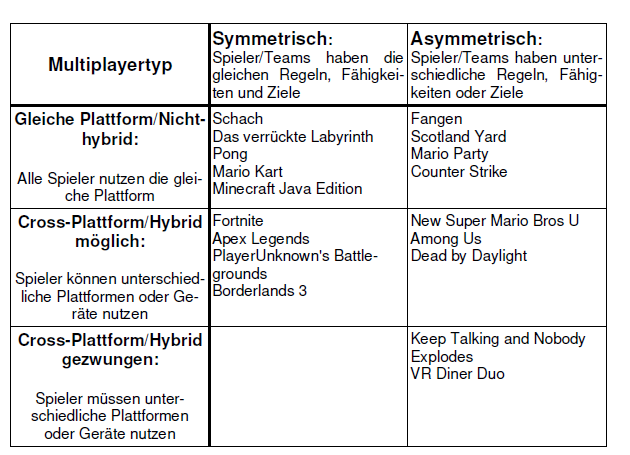
\includegraphics[width=1\linewidth]{content/pictures/lotz_hybrid_multiplayer.PNG}
\caption{Unterscheidung Multiplayertypen nach \cite[S.6]{lotz_konzeption_2021}}
\label{fig:lotz_multiplayer_types}
\end{figure}

Wie Abbildung \ref{fig:lotz_multiplayer_types} zeigt, können Multiplayer-Spiele, auf ihre Medientechnik bezogen, in 3 Kategorien eingeteilt werden.
Spiele wie \say{Mario Kart} oder \say{Minecraft} können nur über die gleiche Plattform gespielt werden. Bei Spielen wie \say{Among Us} oder \say{Fortnite} ist die Plattform, über die gespielt wird, nicht wichtig, da eine Cross-Play-Funktionalität gegeben ist. Jeder kann mit Spielern auf der Plattform spielen, die er bei sich zuhause hat. Die Kategorie ist die, bei der die Spieler gezwungen werden, unterschiedliche Plattformen zu nutzen. In \say{Keep talking and nobody explodes} ist das der Kern des Gamedesigns.

\section{Spielweisen von Multiplayer-Spielen}
Nachdem die unterschiedlichen Strukturen und technischen Formen von Multiplayer-Spielen behandelt wurden, ist es nun wichtig, darauf zu schauen, welche unterschiedlichen Spielweisen sie haben können. Multiplayer-Spiele können dabei in 3 unterschiedliche Spielformen unterschieden werden:
auf competitive, collaborative und cooperative Spielweisen. [Quelle finden]

\subsection{Kompetetiv}
Kompetitive Spiele sind Spiele, bei denen Kombinationen von verschiedenen Spielern gewinnen müssen, während eine andere Kombination von Spielern verlieren oder gemeinsam gewinnen muss. Das Spiel selbst kann weder verlieren noch gewinnen (vgl. \cite{noauthor_game_2014}). [noch andere Quellen suchen]

\subsection{Kollaborativ}
Kollaborative Spiele sind solche, bei denen alle Spieler wie in einem Kooperationsspiel gemeinsam gegen das Spiel verlieren können. Alle zusammen können aber nicht gewinnen. Diese Spiele sind im Kern meist kompetitiv, beinhalten aber die Möglichkeit einer kollektiven Niederlage. Die Spieler müssen zu einem gewissen Maße zusammenarbeiten um nicht zu verlieren (vgl. \cite{noauthor_game_2014}). [noch andere Quellen suchen]

\subsection{Kooperativ}
Bei Kooperationsspielen ist es möglich, dass alle Spieler gemeinsam gegen das Spiel verlieren oder gewinnen können. Ein Sieg wird erreicht, wenn das Spiel gemeinsam \say{besiegt} wird, oder dadurch dass ein festgelegtes Ziel gemeinsam oder individuell erreicht werden konnte (vgl. \cite{noauthor_game_2014}). [noch andere Quellen suchen]

\section{Artverwandte Spiele}
% Hier kommen die analysierten Spiele rein, also die Auflistung der Spiele, die ich mir im Zuge angesehen habe
Nachdem nun die einzelnen Charakteristiken von Multiplayer-Spielen aufgezeigt wurden, werden nun Spiele vorgestellt, welche im Rahmen dieser Arbeit näher betrachtet wurden.

Die Spielreihe \say{\textbf{We were here}} vom niederländischen Entwicklerstudio Total Mayhem Games beinhaltet asymmetrische Kooperative-Multiplayer-Spiele, bei denen zu zweit Rätsel und Hindernisse in der Spielwelt gelöst werden müssen um aus der Umgebung, in denen die Avatare der Spieler gefangen sind, zu entkommen. Dabei können die Spieler über ein \say{In-Game}-Walki-Talki miteinander kommunizieren. Zumeist ist es so, dass ein Spieler verschiedene Rätsel oder Hindernisse für sich hat, die er seinem Mitspieler beschreiben muss, damit dieser die passenden Antworten übermitteln oder Rätsel lösen kann. Die beiden Spieler befinden sich dabei in abgetrennten Räumen oder Gebieten innerhalb der Spielwelt (vgl. \cite{noauthor_we_nodate}; \cite{noauthor_total_nodate}).  

[hier it takes two und split fiction erwähnen]

Das Spiel \say{\textbf{The past within}} vom ebenfalls aus den Niederlanden kommenden Entwicklerstudio Rusty Lake ist ein asymmetrisches kooperatives Multiplayer-Spiel bei dem zwei Spieler gemeinsam in einer Sitzung sowohl in der Vergangenheit als auch in der Zukunft gemeinsam Rätsel lösen müssen um der Protagonistin und ihrem Vater zu helfen. Jeweils ein Spieler befindet sich dabei in einer 2D-Amnwendung, der andere in einer 3D-Anwendung. Es existiert die Möglichkeit, dass das Spiel von verschiedenen Plattformen aus gespielt werden kann (Cross-Plattform Spielbarkeit) (vgl. \cite{noauthor_past_nodate}). 

Das bereits in den vorangegangenen Kapiteln [Kapitel einbinden] erwähnte \say{\textbf{Keep Talking and Nobody Explodes}} ist ein asymmetrisches kooperatives Multiplayer-Spiel bei dem eine Person das Spiel besitzen muss damit es im Team gespielt werden kann. Das Spiel hat eine Besonderheit, da es ein Cross-Plattform Spiel ist, bei dem ein Teilnehmer (der Bombenentschärfer) eine Bombe entschärfen muss und die anderen Spielteilnehmer (die Experten) verschiedene Anleitungen von Bomben vorliegen haben. Die Aufgabe besteht darin die richtige Anleitung für die entsprechende Bombe zu finden und die Bombe innerhalb der vorgegebenen Zeit zu entschärfen. Im Spiel befindet sich jedoch nur der Bombenentschärfer, während die Experten die Anleitungen ausgedruckt durchschauen können (vgl. \cite{noauthor_keep_nodate}).

Im März 2025 erschien das Spiel \say{\textbf{Myrmidon}} vom Studio Studio Popot, welches ein asymmetrischer kooperativer Multiplayer ist, bei dem zwei Spieler zusammen, in zwei verschiedenen Rollen, miteinander spielen können. Eine Rolle ist dabei die Stop-Motion Puppe, welche in einer Stop-Motion Welt Hindernisse überqueren und über verschiedene Plattformen springen muss um ans Ziel zu kommen. Unterstützt wird die Puppe dabei vom Animator, der die Kulisse des Stop-Motion Films bedienen muss, damit die Puppe an ihr Ziel gelangt (vgl. \cite{noauthor_myrmidon_2024}).

\section{Netzwerkinfrastrukturen}
Um ein Multiplayer-Spiel entwickeln zu können, muss zunächst geklärt werden wie die Netzwerk-Infrastruktur der Anwendung auszusehen hat. Es gibt viele verschiedene Ansätze, die für verschiedene Anwendungszwecke gedacht sind.

\subsection{Distributed Authority}
Bei einer \say{Distributed Authority}-Netzwerktopologie übernimmt jeder im Netzwerk verbundene Spielclient gemeinsam jeweils die Verantwortung für das Erstellen und Verwalten von Objekten im Netzwerk. Jeder Client simuliert dabei seinen Teil der Spielwelt selbst und steuert Objekte über seine Autoriät.
Damit Positionen und andere Daten an alle anderen Clients im Netzwerk weitergeleitet werden können, enthält die Topologie einen zentralen und leichtgewichtigen Statusdienst, der diese Funktion übernimmt. Dabei simuliert er die Anwendung nicht, sondern ist nur für die Weiterleitung der nötigen Informationen zuständig (vgl. \cite{noauthor_distributed_2025}).

\begin{figure}[ht]
\centering
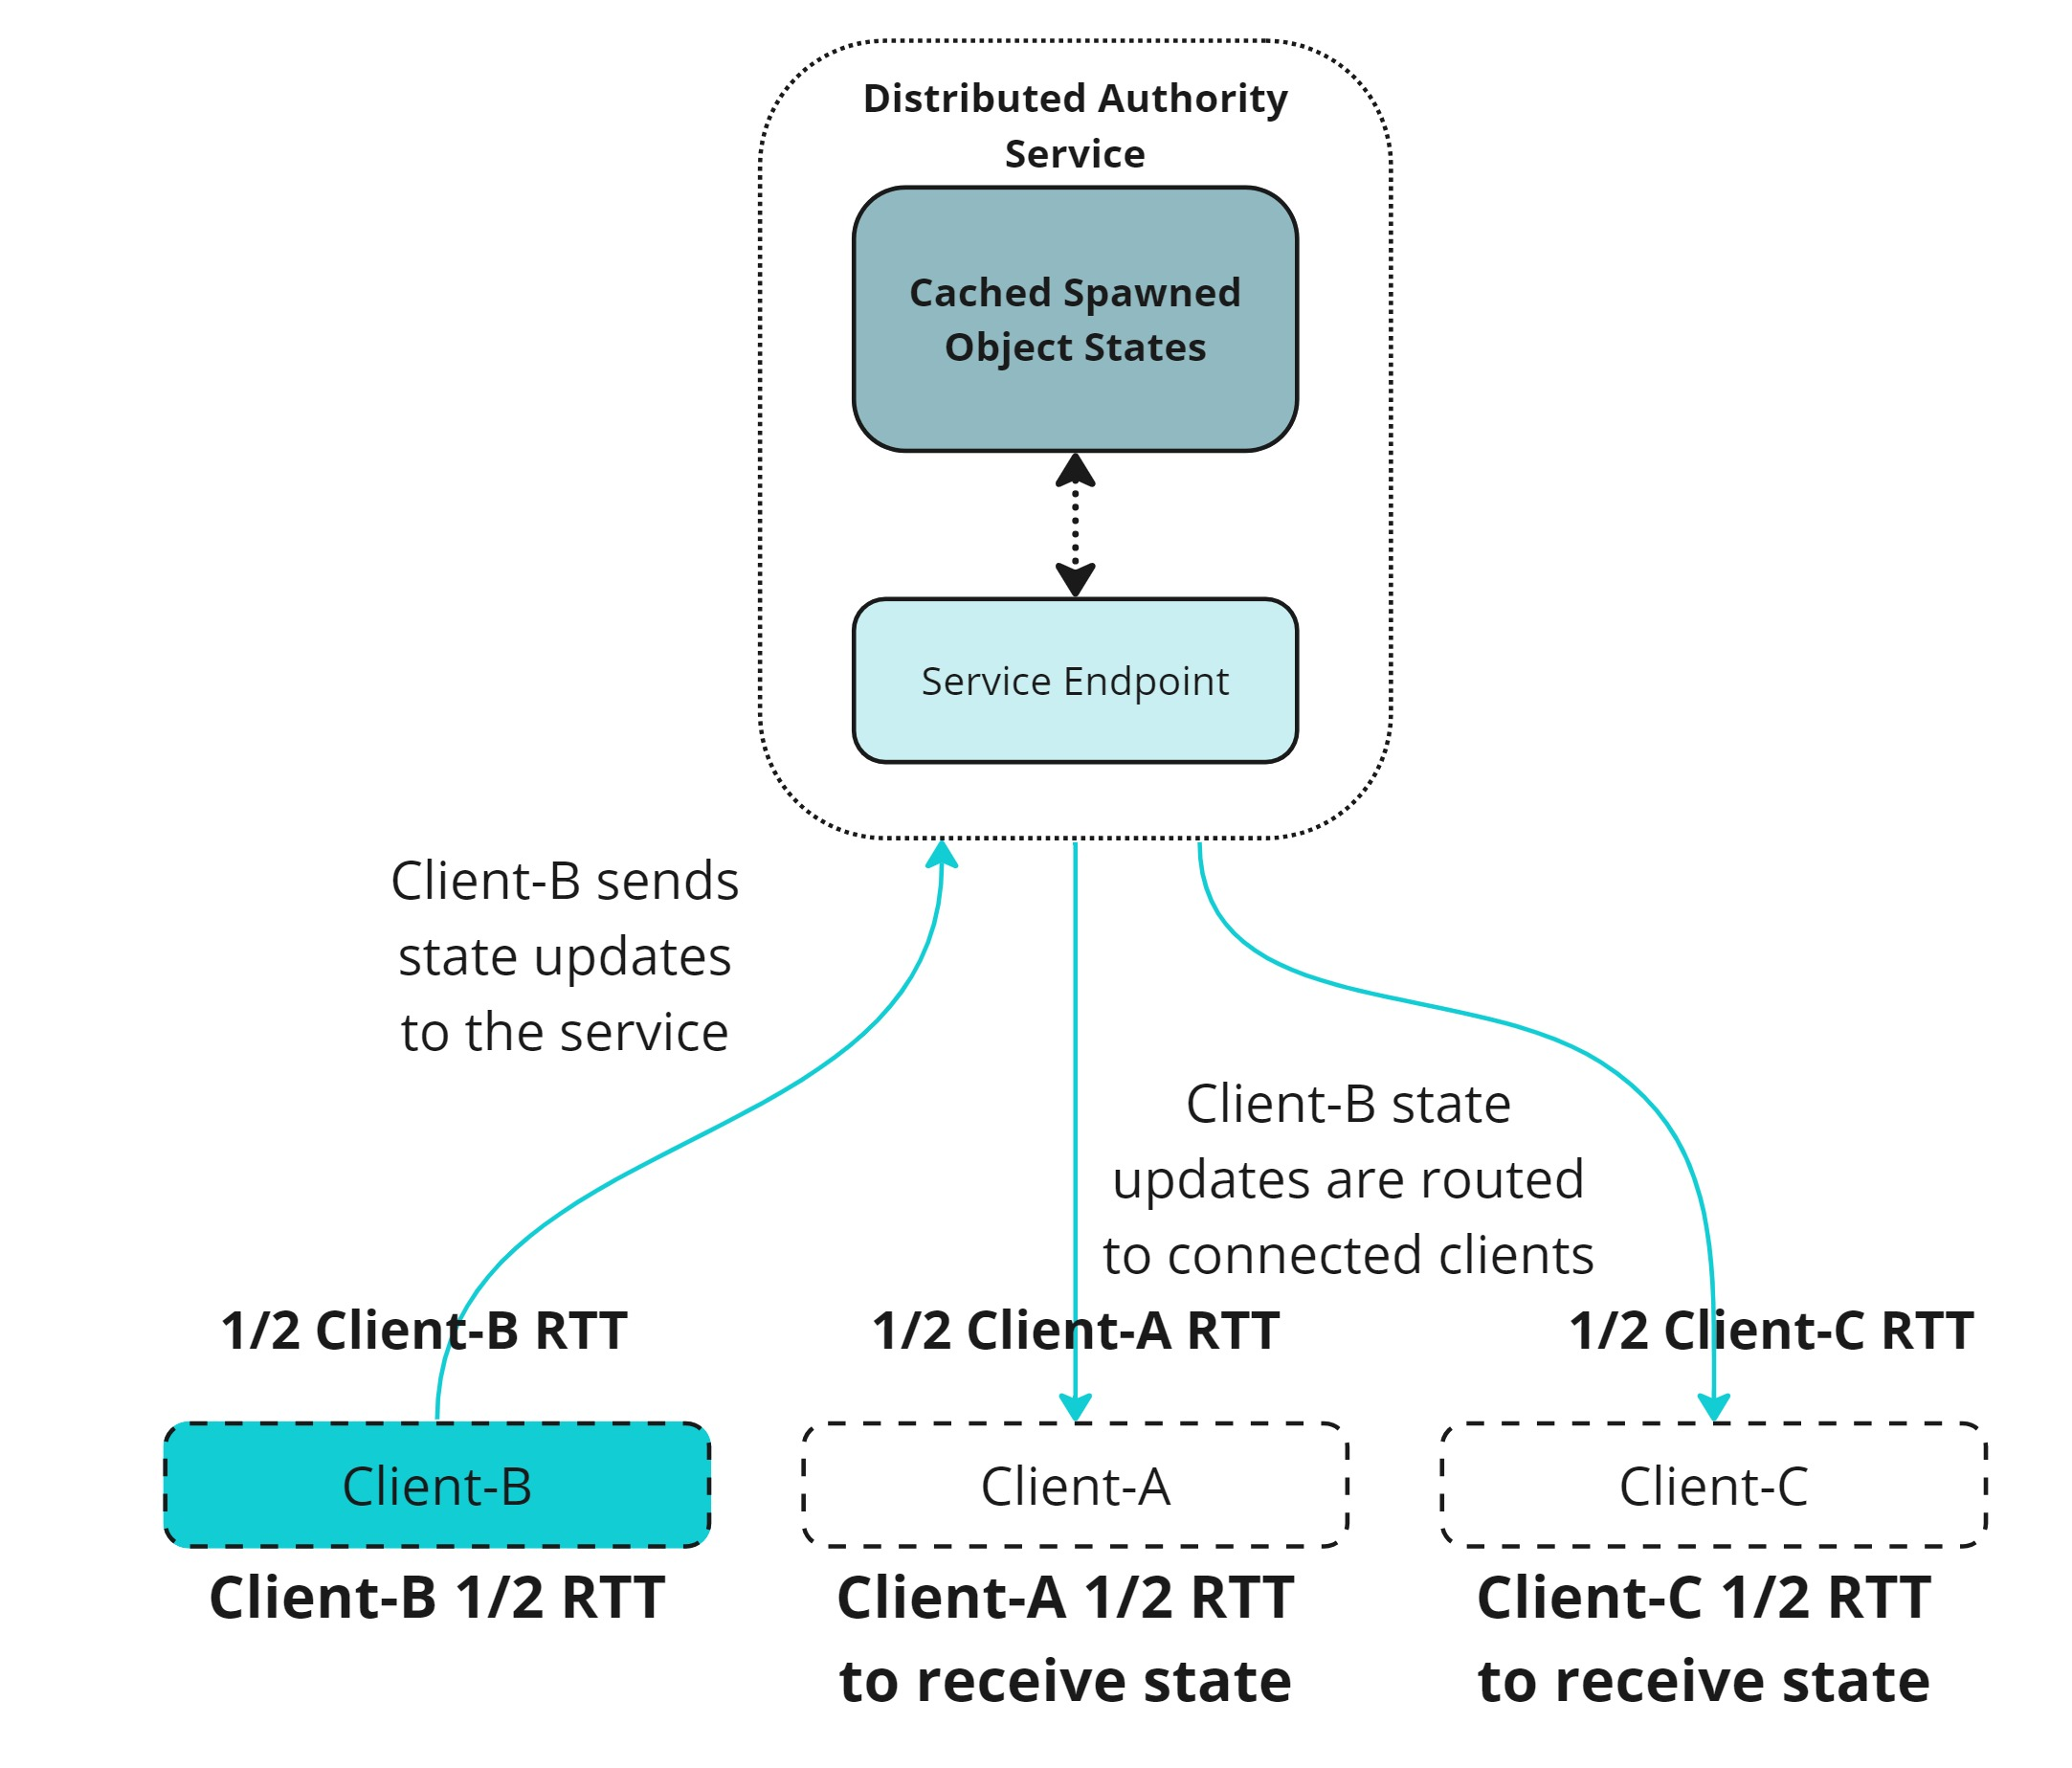
\includegraphics[width=1\linewidth]{content/pictures/distributed-authority-service.jpg}
\caption{Netzwerktopologie der Distributed Authority (vgl. \cite{noauthor_distributed_2025})}
\label{fig:distributed_authority_topology}
\end{figure}

Spiele wie \say{Journey}, \say{God of War: Ascension}, \say{Mercenaries 2}, \say{GTA: Online}, \say{Dark Souls} und \say{Destiny} verwenden diese Netzwerkinfrastruktur. Genutzt wird diese Topologie häufig, wenn ein bestehendes Singleplayer-Spiel eine Multiplayer-Erweiterung erhält (Journey, GTA und Dark Souls), ohne dabei den Kern des Quellcodes umzustrukturieren. Für diesen Anwendungszweck wird kein dedizierter Server gefordert, das Spiel hat eine große, offene Spielwelt (Dark Souls, GTA) und hat keine deterministische Physik bzw. hat kein deterministisches Spielkonzept wodurch eine Integration nicht zu aufwändig wäre. Außerdem empfiehlt es sich bei Spielen zu integrieren, bei denen die Rechner-CPU (bspw. durch die Physik) stark belastet wird. Bei Spielen mit kooperativer Spielmechanik oder leichten kompetitiven Elementen, sowie innovativen Mehrspielermechaniken lohnt es sich, diese Infrastruktur zu wählen (vgl. \cite{noauthor_choosing_2024}).

\subsection{Pure Client/Server}
Bei der Client-Server-Architektur übernimmt ein zentraler Server die Hauptsimulation und verwaltet alle Aspekte des Spiels. Darunter fällt die Physiksimulation, die Erzeugung und Entfernung von Objekten, sowie die Autorisierung von Client-Anfragen. Aus der Sicht der Clients, besitzen diese die Anwendung, mit der sie sich mit dem Server verbinden können, und bekommen über die Verbindung das Spiel zu sehen.
Für diese Infrastruktur gibt es zwei verschiedene Varianten (vgl. \cite{noauthor_client-server_2024}):
\paragraph{Ein dedizierter Server} der eine separate Instanz bildet, welche ausschließlich dem Spielbetrieb dient (vgl. Abbildung \ref{fig:dedicated_server}).

\begin{figure}[ht]
\centering
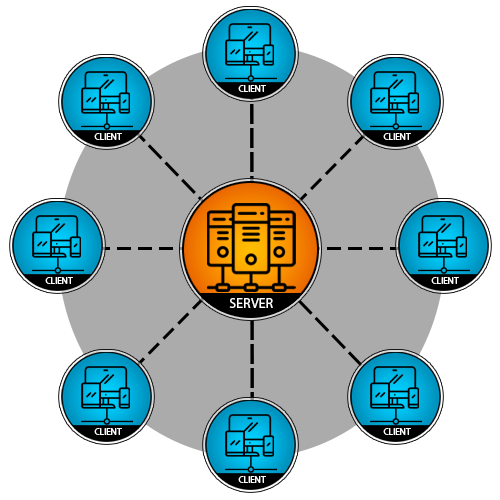
\includegraphics[width=1\linewidth]{content/pictures/ded_server-d5369721966357b9b4d5e1fa96b05b22.png}
\caption{Client-Server-Architektur mit dediziertem Server (vgl. \cite{noauthor_network_2024})}
\label{fig:dedicated_server}
\end{figure}

\paragraph{Client hosted} einen Server und läuft damit auf demselben Gerät wie die entsprechende Client Anwendung (vgl. Abbildung \ref{fig:client_server}).

\begin{figure}[ht]
\centering
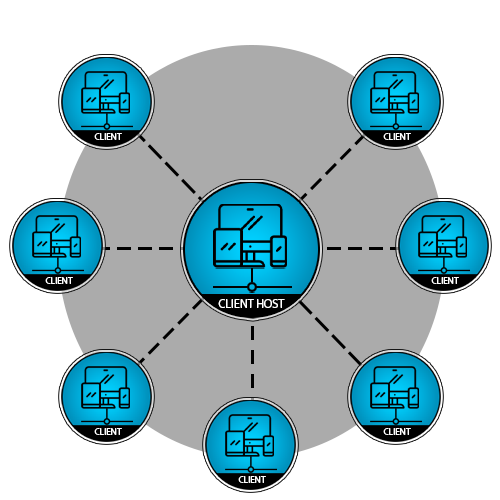
\includegraphics[width=1\linewidth]{content/pictures/client-hosted-16be0b1c9b5020f21325b1e6a7beca73.png}
\caption{Client hosted Server (vgl. \cite{noauthor_network_2024})}
\label{fig:client_server}
\end{figure}

% \subsection{Client-Side Prediction and Lag Compensation}

% Spiele wie \say{Counterstrike}, \say{Call of Duty}, \say{Valorant} und \say{Apex legends} verwenden ein auf dem klassischen Quake-Modell basierendem Netzwerkmodell. Der Spieler steuert dabei lokal im eigenen Client, auf dem die volle Simulation läuft, ohne dabei Verzögerungen beim Laufen oder Schießen zu haben. Der Server nimmt die Eingaben samt Zeitstempel des Clients entgegen und verteilt den \say{State} zurück. Bspw. das Inventar, Munition oder Feuerraten. Die Korrekturen des \say{State}s werden rückwirkend auf den Client angewandt, der den Zustand bis zur aktuellen Zeit wieder herstellt (\say{Client-Side Prediction}). Schüsse und der damit einhergehende Schaden wir auf dem Server ausgewertet und an die Clients übergeben. Um das Spielerlebnis reaktionsschnell und präzise zu gestatlten, nutzt der Server ein \say{Lag Compensation} Verfahren, bei dem er anhand gespeicherter Zustände die Welt aus der Sicht der Clients zum Schlusspunkt rekonstruiert wird (vgl. \say{}.

\subsection{Peer-to-Peer}
Das \ac{P2P}-Architektur-Modell verbindet jeden Spieler mit allen anderen Spielern. Über die Verbindung werden Daten über Spielzustände und Ereignisse ausgetauscht. Im \say{reinen} \ac{P2P}-Sytsme gibt es keinen einzelnen \say{Host}, stattdessen ist jeder Client dafür verantwortlich, einen eigenen Avatar (oder Einheiten) zu veralten und erhält gleichzeitig Updaes der anderen Clients (vgl. \cite{mygames_unity_2024}). Abbildung \ref{fig:p-2-p} zeigt die Topologie.

\begin{figure}[ht]
\centering
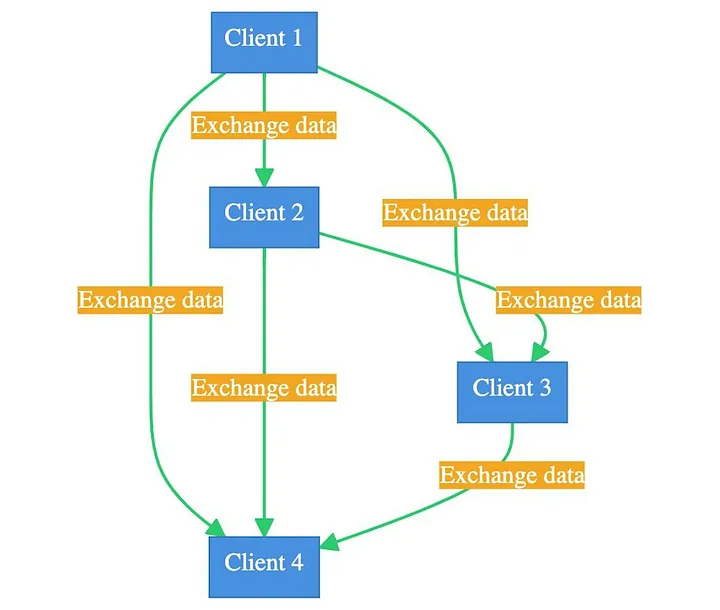
\includegraphics[width=1\linewidth]{content/pictures/0_poGQC2fWQ3tPWPwT.png}
\caption{Peer-to-Peer Infrastruktur (vgl. \cite{mygames_unity_2024}}
\label{fig:p-2-p}
\end{figure}


\subsection{Relay-Server}
Der Relay-Dienst ermöglicht Multiplayer-Unterstützung ohne dedizierten Spielserver. Er übermittelt deshalb die Kommunikation zwischen Spielern über sogenannte Relay-Server. Nachrichten werden zwischen verbundenen Spielern mittels latenzarmer Datagramm-Übertragung übertragen, sodass keine zwei Spieler direkt miteinander verbunden sein müssen (vgl. \cite{noauthor_relay_nodate}).

\begin{figure}[ht]
\centering
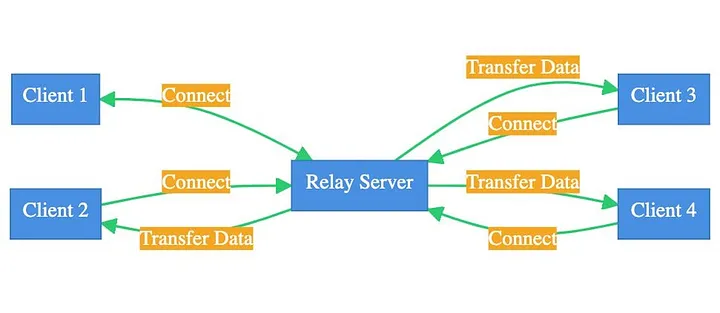
\includegraphics[width=1\linewidth]{content/pictures/0_o7LJU1ImxPHIM5Ej.png}
\caption{Relay-Server Infrastruktur (vgl. \cite{mygames_unity_2024})}
\label{fig:relay-server}
\end{figure}

% \subsection{Verwendete Kommunikationsprotokolle}
% [überlegung hier noch die protokolle erwähnen]

\chapter{Verwandte Arbeiten}\label{sec:related-works}
In der \ac{CSCW} und \ac{HCI} bzw. \ac{CHI} existieren bereits diverse Arbeiten zu Multiplayer-Spielen, Effekt von Computerspiele auf das soziale Beisammensein der Spieler und welche Aspekte aus dem Gamedesign dafür verantwortlich sind.

Im Zentrum steht dabei häufig die Frage, wie Spiele soziale Interaktionen fördern oder hemmen, sowohl im kompeteiven als auch im kollaborativen Kontexten.

Video- und Computerspiele im Allgemeinen können einen positiven Einfluss auf das Miteinander haben. So untersuchte \cite{mason_friends_2013} wie wichtig Freundschaften für den Erfolg von Einzelpersonen und Teams in komplexen kollaborativen Umgebungen sind. Sie fanden heraus, dass Freundschaften einen großen Einfluss auf die verbesserte individuelle- und Teamleistung haben. Spieler richten sich dabei nach sozialen Gelegenheiten aus, sodass verborgene Freundschaftsbeziehungen direkt abgeleitet werden konnten. Kern der Studie war dabei der Online Multiplayer First-Person-Shooter \say{Halo: Reach} bei dem Spieler des Spiels eine anonyme Online Umfrage Fragen ausfüllen mussten. 

Doch soziale Dynamiken verlaufen nicht immer so positiv wie erhofft. Andere Untersuchungen zeigen ein differenzierteres Bild des Zusammenspiels in Onlinewelten.

So argumentiert \cite{ducheneaut_alone_2006} anhand einer Langzeitstudie zu \say{World of Warcraft}, dass soziale Aktivitäten in \ac{MMOG}s, oft überschätzt werden. Die meisten Spieler sind zwar von anderen umgeben, interagieren jedoch nur selten aktiv miteinander. Sie spielen häufig \say{allein zusammen}. Vor allem in den Quests zum Anfang ist das oft der Fall. Erst durch langfristige soziale Strukturen wie Gilden entstehen nachhaltige Bindungen und echte Zusammenarbeit.

Damit jedoch solche sozialen Beziehungen überhaupt entstehen können, ist es essenziell, dass Spiele die Aufmerksamkeit und das Interesse der Spielenden wecken - ein Aspekt, der unter dem Begriff \say{Player Engagement} intensiv erforscht wird.

\cite{rashed_review_2025} fassen in ihrer Überblickasarbeit unterschiedliche Methoden zur Schätzung des Spieler-Engagements zusammen. Ihr Ziel war es, über verschiedene Messmethoden wie EEG, Mimik, Eye Tracking und Spieler-Verhalten hinreichend eindeutige Daten zu sammeln um darüber eine Aussage über das Engagement treffen zu können. Die Validierung der Ergebnisse, da das Engagement subjektiv ist, ist schwer um objektiv eine \say{Ground Truth} Aussage treffen zu können.  \cite{yu_video_2023} verfolgten einen anderen Ansatz. Sie versuchten nicht nur auf das Engagement der Spieler einzugehen, sondern erforschten direkt im Bereich Zusammenarbeit und Kollaborative Fähigkeiten. Sie untersuchten kommerzielle Multiplayer-Spiele um Konzepte und Spielmechaniken zu identifizieren, die von Game-Designern zur Förderung von kooperativen Spielen genutzt werden können. Im Zuge der Forschung entwickelten sie kleine Prototypen und führten mit ihnen kleine Studien durch. 

Einige Studien gehen noch einen Schritt weiter und untersuchten nicht nur Engagement, sondern die spezifischen Bedingungen erfolgreicher Kooperation in Spielen - insbesondere durch das Design asymmetrischer Rollenverteilungen.

So zeigen die Arbeiten von \cite{harris_beam_2014}, \cite{harris_leveraging_2016} und \cite{harris_asymmetry_2019}, dass asymmetrische Spielkonzepte - bei denen sich Rollen, Fähigkeiten und Ziele der Spielenden unterschieden - einen positiven Einfluss auf die Zusammenarbeit hat. Untersucht werden dabei die Faktoren \say{Interdependence}, \say{Degrees of Interdepencene} sowie Mechaniken der Asymmetrie und Abhängigkeiten der Anwendungen. Ein asymmetrisches Spielkonzept ermöglicht außerdem eine Integration bzw. Inklusion von Spielergruppen mit eingeschränkten Fähigkeiten (vgl. \cite{goncalves_exploring_2021}). Für die Entwicklung von Spielen, die für die gesamte Familie gedacht sind, eignet es sich ebenfalls (vgl. \cite{pais_promoting_2024}).

Die Arbeiten von Harris et. al. dienen als Grundlage für die weitere Entwicklung des Game Designs für asymmetrische Multiplayer-Spiele. So identifizierte \cite{guimaraes_rocha_game_2008} verschiedene kooperative Design-Pattern, die in der weiteren Forschung und deren Spielumsetzung anklang fanden. In der Arbeit von \cite{emmerich_impact_2017} werden drei der definierten Pattern verwendet um eine Aussage darüber treffen zu können, wie sich Interaktionen im Spiel gezielt gestalten lassen. Die Ergebnisse der Studie zeigen, dass eine hohe Spielerinterdependenz mit mehr Kommunikation und weniger Frustration einhergeht. Geteilte Kontrolle führte jedoch zu einem geringeren Erleben von Kompetenz und Autonomie.

Diese gestalterischen Grundlagen bilden einen Ausgangspunkt für eine weiterführende Forschung, die sich nun den sozialen, psychologischen und metastrukturellen Wirkungen dieser Spielkonzepte widmet.

Die Arbeit von \cite{depping_trust_2016} beschäftigte sich mit dem zwischenmenschlichen Vertrauen innerhalb einer zusammenarbeitenden Gruppe. Der Fokus lag dabei auf der Problematik, dass im Online-Umfeld bewährte Methodiken zum Teambildung nur schwer umsetzbar sind und bestimmte Situationen einfacher simuliert werden müssen. Daher wurde durch Einsatz eines sozialen Spiels bestimmte Situation wie Risikosituationen und gegenseitige Abhängigkeiten simuliert. Das Zusammenarbeiten im Team kann auch eine Quelle von Konflikten oder Veränderungen sein. \cite{velez_ingroup_2014} zeigen den Fall, dass eine (neue) fremde Person zu einer bestehenden Gruppe Spannungen erzeugen kann. Ihre Studie belegtr, dass kooperative Spiele nicht nur das Helferverhalten steigert, sondern auch das Aggressionsverhalten gegenüber Mitgliedern einer Fremdgruppe verringern kann.

In der Forschung von \ac{VR}-Spielen entstanden einige Interessante Arbeiten bezüglich des Game-Designs aber auch der enthaltenen Forschung.

\cite{karaosmanoglu_playing_2023} untersuchten die Vertrautheit von Zweierteams, die aus sich Fremden oder befreundeten Personen bestanden, im Zusammenhang mit sozialen und spielerischen Erfahrungen sowie ihrer Spielleistung. Die Studie ergab, dass es keine signifikanten Unterschiede zwischen den Freundeteams und Fremdenteams gab. Um Zusammenarbeit ging es ebenfalls in der Anwendung von \cite{sajjadi_maze_2014}. Die Ergebnisse der Studie zeigen, dass das konzipierte Spielkonzept bei den Spieler-Rollen mit den Sifteo Cubes und der VR Anwendung für die Oculus Rift eine positive Bewertung sowohl des Spielerlebnisses als auch der Zusammenarbeit ergab. Ebenfalls mit dem Bezug auf die Zusammenarbeit beschäftigte sich die Arbeit von \cite{smilovitch_birdquestvr_2019}, bei der es darüber hinaus um das Ausschöpfen der Möglichkeiten von \ac{VR} ging.

Im Kerngebiet der Kommunikation beschäftigte sich \cite{nasir_cooperative_2013} und \cite{nasir_effect_2015} zunächst mit der Entwicklung eines \say{ice-breaking} Spiels, das in Form eines 2D-\ac{RPG} konzipiert und entwickelt wurde. Der Sinn des Spiels ist dabei, die Zusammenarbeit in einer folgenden Gruppenarbeit zu verbessern. In der Studie wurden dabei drei unterschiedliche Gruppen miteinander verglichen (eine Gruppe hat das konzipierte Spiel gespielt, eine weitere hatte ein generisches ice-breaking Spiel gespielt und die dritte Gruppe keins). Die Gruppen, die das konzipierte Spiel gespielt hatten, zeigten eine erhöhte Interaktion. Die fortführende Studie untersuchte, ob das aus der ersten Studie umgesetztee Spiel die Zusammenarbeit in realen Teams verbessern kann. Es wurden dabei Gruppen verglichen, die vor der Arbeitsaufgabe das konzipierte ice-breaking gespielt hatten, mit denen, die es nicht gespielt hatten. Es wurde festgestellt, dass die Gruppen, die das ice-breaking Spiel spielten, in der anschließenden Arbeitsaufgabe eine erhöhte Zusammenarbeit zeigten.
% zunächst mit der Wirkung eines kooperativen \say{ice-breaking} Spiel (Kennenlern-Spiel), das als Instrument dienen soll die Zusammenarbeit zu verbessern. Die Ergebnisse der Studie zeigten, dass die Gruppe, die das Kennenlern-Spiel gespielt hatten, mit erhöhter Interaktion an der Folgeaufgabe teilgenommen hatten, als die Vergleichsgruppe. In der darauffolgenden Arbeit 

% Die \ac{AR}-Forschung beschäftigte sich ebenfalls mit 

% [weiterführen dann mit den papern von den design pattern, da die hier dazu kommen, dann beispiele bringen die das als grundlage nehmen im übertragenene sinne]

% Eine der Arbeiten im Themengebiet dieser Arbeit wurde von \cite{nasir_effect_2015}, bei der es darum geht eine \say{Icebreaking}-Anwendung in Form eines Computer- und Videospiels zu haben um erste Hürden im Kennenlernen und effektiven gemeinsamen Arbeiten zu überwinden. Es zeigte sich, dass die Gruppe, die das Icebreaking-Videospiel gespielt hatte, eine erhöhte Zusammenarbeit. [Fortsezen mit inhalt des spiels und dann die forschung beschreiben]

% \cite{harris_asymmetry_2019}
% \cite{sajjadi_maze_2014}

% hier würden Paper reinkommen die asymmetrische Multiplayer gemacht haben, welche aspekte da mitreinspielen, da kommen dann auch die wichtigen Begriffe dazu mitrein. Auch bereits umgesetzt asymetrische VR Spiele?


% Auch Anna Lotz´ Thesis wäre hier relevant


\section{Wichtige Begriffe}
In den vorangegangenen Arbeiten beschäftigten sich die Autoren mit einigen Begrifflichkeiten, die Grundlage in der Konzeption und Entwicklung dieses Prototyps sowie der Forschung dieser Arbeit sind. 

In den folgenden Kapiteln werden diese Begriffe erklärt.

\subsection{Interdependence}
Der Begriff \say{Interdependence} stammt aus dem psychologischen Rahmenwerk für soziale und gruppenbezogene Interaktionen. Die Interdependence wird über das Ausmaß, in dem Gruppenmitglieder aufeinander angewiesen sind, um ihre Aufgabe effektiv zu erfüllen, definiert \cite[S. 451]{depping_cooperation_2017}, \cite{saavedra_complex_1993}, \cite[S. 197:4]{holly_asymmetric_2023}. Auf Video- und Computerspiele bezogen, können Aufgaben als das Spielziel bezeichnet werden \cite[S. 451]{depping_cooperation_2017}. 
In \cite[S. 52]{van_der_vegt_patterns_2001} werden unterschiedliche Formen der Interdependence vorgestellt:
\paragraph{Task interdependence} beschreibt die Abhängigkeit von Teammitgliedern in ihren Aufgaben, die sie zu tun haben. Der Grad der Abhängigkeit nimmt zu, je komplexer die Aufgabe wird.
\paragraph{Goal interdependence} beschreibt die quantitativen und qualitativen Leistungen, die von den Gruppenmitgliedern gemeinsam erreicht werden müssen, um das Gruppenziel zu erreichen.

[Hier schauen ob noch in den anderen Papern was dazu steht]

% \begin{itemize}
% \item \textbf{Task interdependence}: 
%     % \item \textbf{Kann eine spielbasierte Umgebung für die Untersuchung und Verbesserung von Kommunikation zwischen zwei oder mehreren Personen realisiert werden?}
%     % \item \textbf{Welche spezifischen Eigenschaften muss eine solche Umgebung aufweisen und welche Kommunikationsparameter werden dabei angesprochen?}
%     % \item \textbf{Welche Verbesserungen in der Kommunikation zwischen den Anwendern können durch ein asynchrones Multiplayer-Spiel mit zwei verschiedenen Spielerklassen beobachtet werden?}
%     % \item \textbf{Welche Unterschiede können in der Art das Kommunikationsverhalten bei der Verwendung von zwei unterschiedlichen Anwendungen (AR und 3D) (festgestellt/beobachtet) werden}
%     % \item \textbf{Wie stehen die Nutzer zu einem spielerischen Ansatz und zur Verbesserung der Kommunikation, insbesondere auch im Umgang mit Fremden?}
% \end{itemize}
% \cite{harris_leveraging_2016}
% \cite{depping_cooperation_2017}

\subsection{Degrees of Interdependence}
In der Arbeit von \cite[S. 7]{harris_asymmetry_2019} werden unterschiedliche Grade der Interdependence untersucht. Unter Grad der interdependence versteht man das Ausmaß in dem die Handlungen der Spieler voneinander abhängig sind, um das Spielziel erfolgreich zu erreichen. Je höher der Grad der Interdependence, desto stärker sind die Spieler darauf angewiesen, sich gegenseitig abzustimmen zusammenzuarbeiten um ihre Handlungen aufeinander abzustimmen (vgl. \cite[S. 7]{harris_asymmetry_2019}.

[Hier schauen ob noch in den anderen Papern was dazu steht]

% \cite{beznosyk_effect_2012}

\subsection{Soziale Präsenz}
Die soziale Präsenz beschreibt \say{das Gefühl, mit einem anderen zusammen zu sein} [eigene Übersetzung] \cite[S. 1]{biocca_towards_2003}. \say{Das andere} kann dabei entweder ein anderer Mensch oder eine künstliche Intelligenz sein. Innerhalb der \ac{HCI} untersucht die Theorie der sozialen Präsenz, wie das \say{Gefühl, mit einem anderen anderen zusammen zu sein} [eigene Übersetzung] \cite[S. 1]{biocca_towards_2003} durch Schnittstellen gestaltet und beeinflusst wird (vgl. \cite[S. 1]{biocca_towards_2003}). Sie wird im Einzelnen durch die Wahrnehmung der physischen Repräsentation des anderen Spielers sowie durch psychologische Beteiligung und Verhaltensabhängigkeiten gekennzeichnet. Soziale Präsenz kann somit als das Ergebnis eines komplexen Zusammenspiels von wechselseitigem Verhalten, Kommunikation und sozialen Kontextmerkmalen gesehen werden. Die Voraussetzung hierfür ist, dass ein Spieler die Kopräsenz einer anderen sozialen Einheit wahrnimmt (vgl. \cite[S. 1]{emmerich_game_2016}).#

[Hier schauen ob noch in den anderen Papern was dazu steht]

% \cite{emmerich_impact_2017}

% Vertrauen gibts in dem Kontext auch und wie man dan über Spiele aufbaut

\section{Untersuchungsschwerpunkte}
In diesem Kapitel wird der Untersuchungsschwerpunkt dieser Arbeit vorgestellt. Dabei wird Bezug auf die bestehende Forschung aus dem Kapitel \emph{\nameref{sec:related-works}} genommen.

Diese Arbeit greift die grundlegende Forschung der Arbeiten von Nassir in \cite{nasir_cooperative_2013} und \cite{nasir_effect_2015} auf und erweitert diese durch Vor- und Nachtests derselben Versuchsgruppe, um zu beweisen, dass eine bestehende Gruppe durch die Anwendung des erstellten Prototyps gezielt in der gemeinsamen Kommunikation verbessert werden kann. Der Prototyp dient zudem nicht als stilisierte Anwendung für den Zweck des Ice-Breakings, sondern auch als Multiplayer-Spiel, das in der Freizeit gespielt werden kann.

Hinzu kommt, dass die Anwendung ein \say{Cross-Plattform} Multiplayer (vgl. Abbildung: \ref{fig:lotz_multiplayer_types}) ist, bei dem unterschiedliche Plattformen genutzt werden müssen und die damit einhergehende Wirkung mit untersucht werden soll. Im Fokus steht dabei die \ac{AR}-Integration einer Anwendung und die Touchsteuerung beider Anwendungen, die im Prototyp umgesetzt werden sollen.
